\documentclass[a4paper, 14pt]{extarticle}
\usepackage{float}
% Поля
%--------------------------------------
\usepackage{geometry}
\geometry{a4paper,tmargin=2cm,bmargin=2cm,lmargin=3cm,rmargin=1cm}
%--------------------------------------


%Russian-specific packages
%--------------------------------------
\usepackage[T2A]{fontenc}
\usepackage[utf8]{inputenc} 
\usepackage[english, main=russian]{babel}
%--------------------------------------

\usepackage{textcomp}

% Красная строка
%--------------------------------------
\usepackage{indentfirst}               
%--------------------------------------             


%Graphics
%--------------------------------------
\usepackage{graphicx}
\graphicspath{ {./images/} }
\usepackage{wrapfig}
%--------------------------------------

% Полуторный интервал
%--------------------------------------
\linespread{1.3}                    
%--------------------------------------

%Выравнивание и переносы
%--------------------------------------
% Избавляемся от переполнений
\sloppy
% Запрещаем разрыв страницы после первой строки абзаца
\clubpenalty=10000
% Запрещаем разрыв страницы после последней строки абзаца
\widowpenalty=10000
%--------------------------------------

%Списки
\usepackage{enumitem}

%Подписи
\usepackage{caption} 

%Гиперссылки
\usepackage{hyperref}

\hypersetup {
	unicode=true
}

%Рисунки
%--------------------------------------
\DeclareCaptionLabelSeparator*{emdash}{~--- }
\captionsetup[figure]{labelsep=emdash,font=onehalfspacing,position=bottom}
%--------------------------------------

\usepackage{tempora}

%Листинги
%--------------------------------------
\usepackage{listings}
\lstset{
  basicstyle=\ttfamily\footnotesize, 
  %basicstyle=\footnotesize\AnkaCoder,        % the size of the fonts that are used for the code
  breakatwhitespace=false,        % sets if automatic breaks shoulbd only happen at whitespace
  breaklines=true,                 % sets automatic line breaking
  captionpos=t,                    % sets the caption-position to bottom
  inputencoding=utf8,
  frame=single,                    % adds a frame around the code
  keepspaces=true,                 % keeps spaces in text, useful for keeping indentation of code (possibly needs columns=flexible)
  keywordstyle=\bf,       % keyword style
  numbers=left,                    % where to put the line-numbers; possible values are (none, left, right)
  numbersep=5pt,                   % how far the line-numbers are from the code
  xleftmargin=25pt,
  xrightmargin=25pt,
  showspaces=false,                % show spaces everywhere adding particular underscores; it overrides 'showstringspaces'
  showstringspaces=false,          % underline spaces within strings only
  showtabs=false,                  % show tabs within strings adding particular underscores
  stepnumber=1,                    % the step between two line-numbers. If it's 1, each line will be numbered
  tabsize=2,                       % sets default tabsize to 8 spaces
  title=\lstname                   % show the filename of files included with \lstinputlisting; also try caption instead of title
}
%--------------------------------------

%%% Математические пакеты %%%
%--------------------------------------
\usepackage{amsthm,amsfonts,amsmath,amssymb,amscd}  % Математические дополнения от AMS
\usepackage{mathtools}                              % Добавляет окружение multlined
\usepackage[perpage]{footmisc}
%--------------------------------------

%--------------------------------------
%			НАЧАЛО ДОКУМЕНТА
%--------------------------------------

\begin{document}

%--------------------------------------
%			ТИТУЛЬНЫЙ ЛИСТ
%--------------------------------------
\begin{titlepage}
\thispagestyle{empty}
\newpage


%Шапка титульного листа
%--------------------------------------
\vspace*{-60pt}
\hspace{-65pt}
\begin{minipage}{0.3\textwidth}
\hspace*{-20pt}\centering

\includegraphics[width=\textwidth]{emblem}
\end{minipage}
\begin{minipage}{0.67\textwidth}\small \textbf{
\vspace*{-0.7ex}
\hspace*{-6pt}\centerline{Министерство науки и высшего образования Российской Федерации}
\vspace*{-0.7ex}
\centerline{Федеральное государственное бюджетное образовательное учреждение }
\vspace*{-0.7ex}
\centerline{высшего образования}
\vspace*{-0.7ex}
\centerline{<<Московский государственный технический университет}
\vspace*{-0.7ex}
\centerline{имени Н.Э. Баумана}
\vspace*{-0.7ex}
\centerline{(национальный исследовательский университет)>>}
\vspace*{-0.7ex}
\centerline{(МГТУ им. Н.Э. Баумана)}}
\end{minipage}
%--------------------------------------

%Полосы
%--------------------------------------
\vspace{-25pt}
\hspace{-35pt}\rule{\textwidth}{2.3pt}

\vspace*{-20.3pt}
\hspace{-35pt}\rule{\textwidth}{0.4pt}
%--------------------------------------

\vspace{1.5ex}
\hspace{-35pt} \noindent \small ФАКУЛЬТЕТ\hspace{80pt} <<Информатика и системы управления>>

\vspace*{-16pt}
\hspace{47pt}\rule{0.83\textwidth}{0.4pt}

\vspace{0.5ex}
\hspace{-35pt} \noindent \small КАФЕДРА\hspace{50pt} <<Теоретическая информатика и компьютерные технологии>>

\vspace*{-16pt}
\hspace{30pt}\rule{0.866\textwidth}{0.4pt}
  
\vspace{11em}

\begin{center}
\Large {\bf Лабораторная работа № 1} \\ 
\large {\bf по курсу <<Разработка мобильных приложений>>} \\
\large <<Графический пользовательский интерфейс в Dart>> 
\end{center}\normalsize

\vspace{8em}


\begin{flushright}
  {Студент группы ИУ9-71Б Баев Д.А \hspace*{15pt}\\ 
  \vspace{2ex}
  Преподаватель Посевин Д. П.\hspace*{15pt}}
\end{flushright}

\bigskip

\vfill
 

\begin{center}
\textsl{Москва 2023}
\end{center}
\end{titlepage}
%--------------------------------------
%		КОНЕЦ ТИТУЛЬНОГО ЛИСТА
%--------------------------------------

\renewcommand{\ttdefault}{pcr}

\setlength{\tabcolsep}{3pt}
\newpage
\setcounter{page}{2}

\section{Задание}\label{Sect::task}
В течение лабораторной работы нужно разработать программу, рисующую на экране
мобильного устройства одно из изображений, перечисленных в таблице ниже. Программа
должна иметь графический пользовательский интерфейс, через который пользователь может
задавать параметры изображения. Изображение должно перерисовываться автоматически при
изменении любого параметра. Значения параметров, обозначенных в таблице латинскими
буквами, представляют собой неотрицательные целые числа. Когда в описании изображения
говорится о выборе цвета, подразумевается выбор из нескольких предопределённых
альтернатив (например, красный, зелёный или синий).


Треугольник, заданный сторонами a, b и c, закрашенный цветом,
компоненты R, G и B которого зависят от величины углов треугольника
(угол 0 соответствует величине 0 компоненты, а угол 180 – величине 255).
\newpage
\section{Исходный код}

Исходный код программы представлен в листинге~\ref{lst:code1}

\begin{figure}[H]
\begin{lstlisting}[language={},caption={Реализация мобильного приложения},label={lst:code1}]
import 'package:flutter/material.dart';
import 'dart:math';

void main() {
  runApp(MyApp());
}

class MyApp extends StatelessWidget {
  @override
  Widget build(BuildContext context) {
    return MaterialApp(
      home: MyTriangleApp(),
    );
  }
}

class MyTriangleApp extends StatefulWidget {
  @override
  _MyTriangleAppState createState() => _MyTriangleAppState();
}

class _MyTriangleAppState extends State<MyTriangleApp> {
  double sideA = 100.0;
  double sideB = 100.0;
  double sideC = 100.0;

  @override
  Widget build(BuildContext context) {
    return Scaffold(
      appBar: AppBar(
        title: Text('Triangle Drawer'),
      ),
      body: Column(
        mainAxisAlignment: MainAxisAlignment.center,
        children: [
          TriangleWidget(sideA, sideB, sideC),
          SizedBox(height: 20),
          Text('Side A: ${sideA.toInt()}'),
          Slider(
            value: sideA,
            onChanged: (value) {
              setState(() {
                sideA = value;
              });
            },
            min: 75,
            max: 145,
          ),
          SizedBox(height: 20),
          Text('Side B: ${sideB.toInt()}'),
          Slider(
            value: sideB,
            onChanged: (value) {
              setState(() {
                sideB = value;
              });
            },
            min: 75,
            max: 145,
          ),
          SizedBox(height: 20),
          Text('Side C: ${sideC.toInt()}'),
          Slider(
            value: sideC,
            onChanged: (value) {
              setState(() {
                sideC = value;
              });
            },
            min: 75,
            max: 145,
          ),
        ],
      ),
    );
  }
}

class TriangleWidget extends StatelessWidget {
  final double sideA, sideB, sideC;

  TriangleWidget(this.sideA, this.sideB, this.sideC);

  @override
  Widget build(BuildContext context) {
    double angleA = calculateAngle(sideA, sideB, sideC);
    double angleB = calculateAngle(sideB, sideA, sideC);
    double angleC = 180 - angleA - angleB;

    int colorR = ((angleA / 180) * 255).toInt();
    int colorG = ((angleB / 180) * 255).toInt();
    int colorB = ((angleC / 180) * 255).toInt();

    return Container(
      margin: EdgeInsets.symmetric(vertical: 20),
      child: CustomPaint(
        painter: TrianglePainter(colorR, colorG, colorB, sideA, sideB, sideC, radians(angleA), radians(angleB), radians(angleC)),
        child: Container(
          height: 200,
          width: 200,
        ),
      ),
    );
  }

  double calculateAngle(double a, double b, double c) {
    return degrees(acos((b * b + c * c - a * a) / (2 * b * c)));
  }

  double degrees(double radians) {
    return radians * (180 / pi);
  }

  double radians(double degrees) {
    return degrees * (pi / 180);
  }
}

class TrianglePainter extends CustomPainter {
  final int colorR, colorG, colorB;
  final double sideA, sideB, sideC, angleA, angleB, angleC;

  TrianglePainter(this.colorR, this.colorG, this.colorB, this.sideA, this.sideB, this.sideC, this.angleA, this.angleB, this.angleC);

  @override
  void paint(Canvas canvas, Size size) {
    Paint paint = Paint()
      ..color = Color.fromARGB(255, colorR, colorG, colorB)
      ..style = PaintingStyle.fill;


    Path path = Path();
    path.moveTo(0, 0);
    path.lineTo(sideA, 0);
    path.lineTo(sideC * cos(angleB), sideC * sin(angleB));

    path.close();

    canvas.drawPath(path, paint);
  }

  @override
  bool shouldRepaint(CustomPainter oldDelegate) {
    return true;
  }
}
\end{lstlisting}
\end{figure}


\section{Результаты}

Результаты приведен на рисунках~\ref{fig:img1}-~\ref{fig:img3}

\begin{figure}[H]
\centering
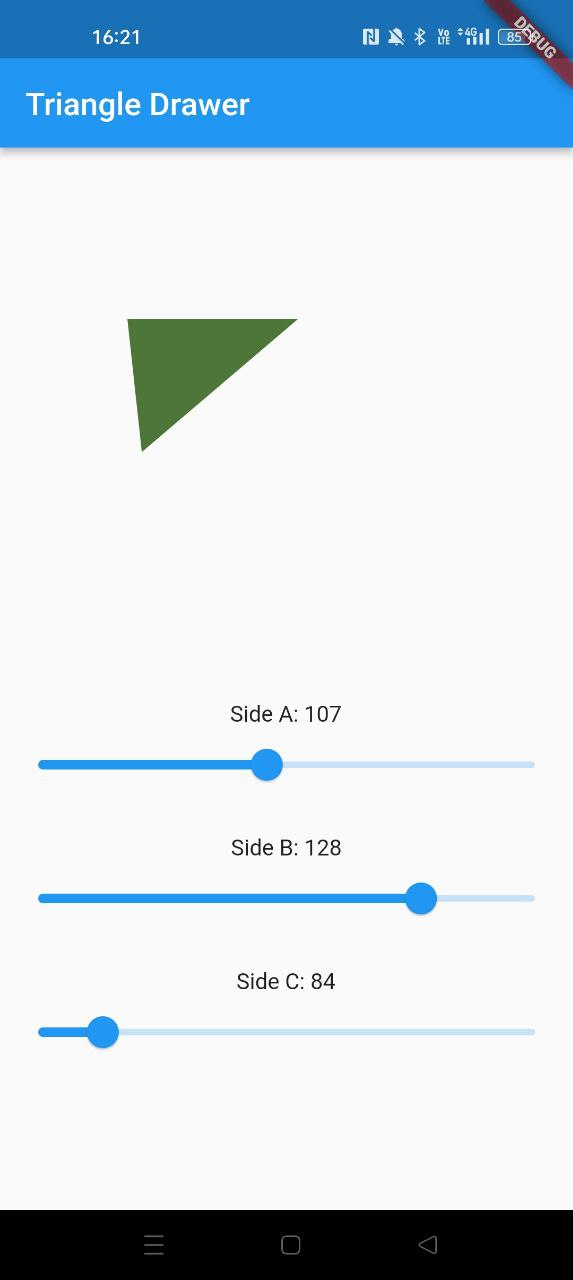
\includegraphics[width=0.5\textwidth]{images/res1.jpg}
\caption{Результат работы мобильного приложения}
\label{fig:img1}
\end{figure}

\begin{figure}[H]
\centering
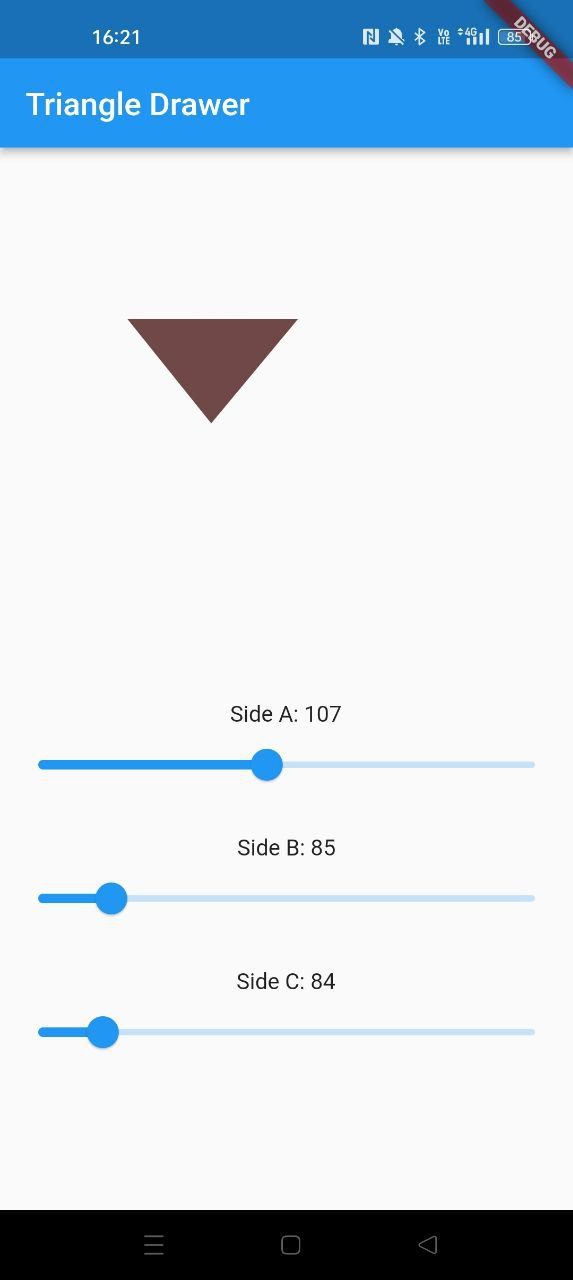
\includegraphics[width=0.5\textwidth]{images/res2.jpg}
\caption{Результат работы мобильного приложения}
\label{fig:img2}
\end{figure}

\begin{figure}[H]
\centering
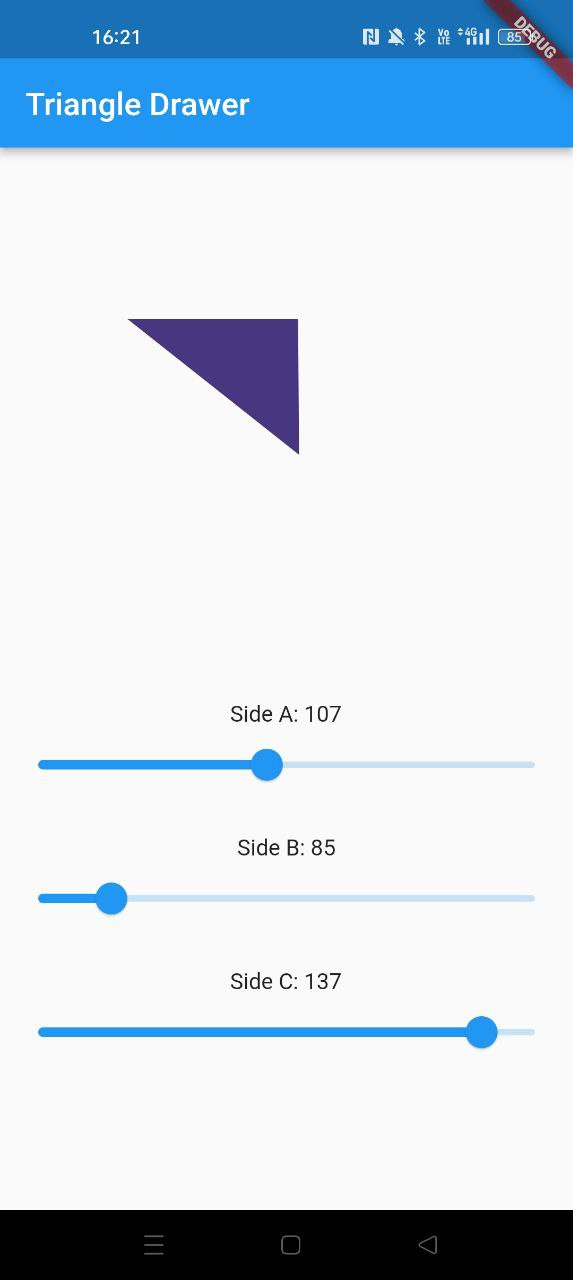
\includegraphics[width=0.5\textwidth]{images/res3.jpg}
\caption{Результат работы мобильного приложения}
\label{fig:img3}
\end{figure}


\section{Выводы}
В рамках данной лабораторной работы произошло знакомство с реализацией графического пользовательского интерфейса в Flutter.
\end{document}
